\documentclass{beamer}
\usepackage{Mydef}
%\usepackage{titlesec}
%\usepackage[left=1in,right=1in,top=1in,bottom=1in]{geometry}
\usepackage[style=alphabetic,backend=bibtex,sorting=nyt,maxcitenames=5,maxbibnames=99]{biblatex}
\addbibresource{reference.bib}


\usetheme{Darmstadt}
\usecolortheme{whale}
\usefonttheme{professionalfonts}


\title[]{Optimization over Orbit Closures of \\ Real Reductive Lie Group Actions}

\author[Zhan Zhiyuan]{Zhan Zhiyuan \\ {\small Associate Prof. Hiroshi Hirai}}
\date{\today}

\begin{document}
	\frame{\titlepage}

	\begin{frame}
		\tableofcontents
	\end{frame}
	
	\AtBeginSection[]{
		\begin{frame}
			\tableofcontents[currentsection]
		\end{frame}
	}

	\section{Introduction}
	\begin{frame}{Matrix Scaling [Sinkhorn\nocite{key14} 1964]}
		Given $A = (a_{ij}) \in M_n(\R)$ with $a_{ij} \geqslant 0$, 
		\begin{itemize}
			\item $A$ is \emph{almost doubly stochastic scalable} if $\forall$ $\varepsilon > 0$, $\exists~$ positive diagonal $X,Y$ s.t. $B = XAY$ satisfies
 			\begin{equation*}
 				\norm{B\mathds{1}- \mathds{1}}_2 < \varepsilon,~\norm{B^T\mathds{1}- \mathds{1}}_2 < \varepsilon
 			\end{equation*}
 			where $\mathds{1} = (1,\cdots,1)^T \in \R^n$.
		\end{itemize}
		\emph{Remark:} In short, we say $A$ is almost scalable.
		\vspace{0.5em}
		\begin{thm}[Rothblum and Schneider\nocite{key1} 1989]
 			$A$ is almost scalable if and only if for every zero minor $I \times J$ of $A$,
 			\vspace{-0.5em}
 			\begin{equation*}
 				\abs{I} + \abs{J} \leqslant n
 			\end{equation*}
 		\end{thm}
	\end{frame}

	\begin{frame}{Connection with Graph Theory}
		Given $A = (a_{ij}) \in M_n(\R)$:
		\vspace{0.5em}
		\begin{itemize}
			\item Bipartite graph $G_A = \bc{[n]\cup[n],E}$: $(i,j) \in E ~\Leftrightarrow~ a_{ij} \neq 0$;
				\begin{center}
					\begin{tabular}{rcl}
						$A = \begin{pmatrix}
							1 & 1 & 1 \\
							1 & 0 & 0 \\
							1 & 0 & 0
							\end{pmatrix}$&
							$\Rightarrow$&
							\begin{tikzpicture}[baseline=-9mm]
						    \graph[nodes={draw,circle,fill=black,inner sep=0pt, minimum size=0.1cm},
						           empty nodes, branch down=0.8 cm,
						           grow right sep=1.2cm] {subgraph I_nm [V={a, b, c}, W={1,...,3}];
										  a[label={\tiny 1}] -- { 1[label={\tiny 1}], 2[label={\tiny 2}], 3[label={\tiny 3}]};
										  b[label={\tiny 2}] -- { 1[label={\tiny 1}] };
										  c[label={\tiny 3}] -- { 1[label={\tiny 1}] }
										};
							\end{tikzpicture}
					\end{tabular}
				\end{center}
			\item Hall's theorem: $G_A$ has a perfect matching $\Leftrightarrow$ 
							\begin{tikzpicture}[baseline=-2mm]
						    	\begin{scope}
							    	\node {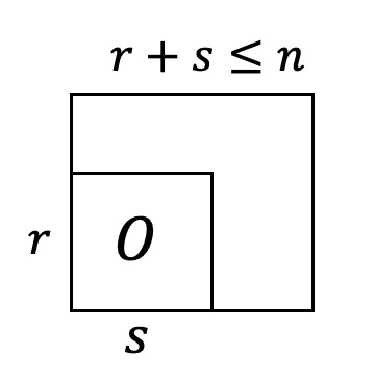
\includegraphics[scale=0.35]{f1.eps}};
							    \end{scope}
							\end{tikzpicture}
			\item \cite{key1}:  $G_A$ has a perfect matching $\Leftrightarrow$ $A$ is almost scalable
		\end{itemize}
	\end{frame}

	\begin{frame}{From Invariant Theory}
		Let $G = ST(n) \times ST(n)$ act on $V = M(n,\R)$, that is
		\vspace{-0.5em}
		\begin{center}
			\begin{tabular}{rrcl}
				$\pi \colon$ & $G$ & $\longrightarrow$ & $GL(V)$
			\end{tabular}
		\end{center}
		\vspace{-0.5em}
		where $ST(n) = \bb{\diag\left(t_1,\cdots,t_n\right) \colon t_j \in \R \backslash \bb{0},~\prod_{j=1}^n t_j = 1}$. 
		\begin{equation*}
			\pi(X,Y)A \defeq XAY,~\forall~(X,Y) \in G
			\vspace{-1.5em}
		\end{equation*}
		\begin{block}{Problem: Null Cone Membership}
			\begin{equation*}
				0 \in \clo{\pi(G)A}?
				\vspace{0.5em}
			\end{equation*}
		\end{block}
		\vspace{0.5em}
		By Hilbert-Mumford Criterion \cite{key2,key3} and \cite{key1},
		\begin{block}{Invariant Theoretic View}
			\begin{center}
				$A$ is almost scalable $\Leftrightarrow$ $0 \notin \clo{\pi(G)A}$.
			\end{center}
		\end{block}
	\end{frame}

	\begin{frame}{Optimization over Orbit Closure}
		The \emph{Kempf-Ness function} of $A = (a_{ij}) \in M_n(\R)$,
		\begin{equation*}
			f_A(x,y) = \log \bc{\frac{\bc{x^TAy}^n}{\prod_{i=1}^nx_i \prod_{j=1}^ny_j}} \colon (\R^+)^{n} \times (\R^+)^{n} \sto \R
		\end{equation*}
		\begin{itemize}
			\item $0 \notin \clo{\pi(G)A}~\Leftrightarrow~\inf f_A > -\infty$
			\item$x_i = e^{s_i},~y_j = e^{t_j}$,
			\vspace{-0.5em}
			\begin{equation*}
				\nabla f_A(s,t)\sim \text{const} \times \bc{\text{Row sums}-\mathds{1},\text{Column sums}-\mathds{1}}
				\vspace{-0.5em}
			\end{equation*}
		\end{itemize}
		\begin{block}{Observation}
			\vspace{-1em}
			\begin{equation*}
				A \text{ is almost scalable} ~\Leftrightarrow~ \inf f_A > -\infty ~\Leftrightarrow~ 0 \in \clo{\nabla f\bc{\R^n \times \R^n}}
				\vspace{0.5em}
			\end{equation*}
		\end{block}
	\end{frame}

	\begin{frame}{Operator Scaling [Gurvits\nocite{key15} 2004]}
		Let $G = SL(n,\C) \times SL(n,\C)$ act $V = M(n,\C)^{\oplus m}$ by
		\begin{equation*}
			\pi(g,h) (A_1,\cdots,A_m) \defeq (gA_1h^{\dagger},\cdots,gA_mh^{\dagger})
		\end{equation*}
		$A = (A_1,\cdots,A_m)$ is \emph{almost scalable} for if $\forall~\varepsilon > 0,~\exists~g,h$ s.t.
		\begin{equation*}
			\norm{\sum_{i=1}^mgA_ih^{\dagger}hA_i^{\dagger}g^{\dagger}-I_n}_{\Fr} < \varepsilon,~\norm{\sum_{i=1}^mhA_i^{\dagger}g^{\dagger}gX_ih^{\dagger}-I_n}_{\Fr} < \varepsilon
		\end{equation*}
	
		Also by Hilbert-Mumford Criterion,
		\begin{thm}[Garg et al.\nocite{key13} 2020]
			\begin{center}
				$A$ is almost scalable $\Leftrightarrow$ $0 \notin \clo{\pi(G)A}$.
			\end{center}
		\end{thm}
	\end{frame}

	\begin{frame}
	 		\textbf{Optimization:} Given $A = (A_1,\cdots,A_m)$,
			\begin{equation*}
				f_A(g,h) = \log \norm{\pi(g,h)A},~g,h \in SL(n,\C)
			\end{equation*}
			where  $\norm{A}^2 = \sum_i \norm{A_i}_F^2$.
			\begin{thm}[\cite{key13}]
				\begin{center}
					$A \text{ is almost scalable } ~\Leftrightarrow~ 0 \in \clo{\nabla f_A(G)} ~\Leftrightarrow~ \inf f_A > -\infty$
				\end{center}
			\end{thm}
			\textbf{Applications:} 
			\begin{itemize}
				\item Noncommutative PIT \cite{key13}:
				\vspace{-0.5em}
				\begin{equation*}
					p(x_1,\cdots,x_n): x_ix_j \neq x_jx_i~\Rightarrow~ p(x_1,\cdots,x_n) = 0?
					\vspace{-0.5em}
				\end{equation*}
				\item Brascamp–Lieb inequalities \cite{key22}: 
				\vspace{-0.5em}
				\begin{equation*}
					\int_{\R^n} \prod_{i=1}^mf_i\bc{B_i(x)} dx \leqslant C \prod_{i=1}^m \norm{f_i}_{1/p_i}
					\vspace{-0.5em}
				\end{equation*}
			\end{itemize}
	\end{frame}

	\begin{frame}{Generalization\nocite{key8} [{\small B{\"u}rgisser,Franks,Garg,Oliveira,Walter and Wigderson 2019}]}
		\begin{itemize}
			\item $G \subset GL(n,\C)$: complex reductive group
			\item $V \simeq \C^m$ and $\pi \colon V \sto GL(V)$: Given $0 \neq v \in V$
		\end{itemize}
		\begin{block}{Problems}
			\begin{itemize}
				\item \textbf{Null cone membership:} determine if $0 \in \clo{\pi(G)v}$
				\item \textbf{Norm minimization:} find $g$ s.t. $\norm{\pi(g)v} \sto \inf \norm{\pi(g)v}$
				\item \textbf{Scaling problem:} Kempf-Ness function $f_v$ $\leadsto$ gradient $\nabla f_v$
				\vspace{-0.5em}
				\begin{equation*}
					\text{find } g \text{ s.t. } \nabla f_v(g) \sto 0
				\end{equation*}
			\end{itemize}
		\end{block}
		\begin{block}{Applications}
			\begin{itemize}
				\item Horn’s problem: $A,B$ Hermitians $\Rightarrow$ eigenvalues of $A+B$
				\item Quantum marginal, Orbit problems, invariant theory, $\cdots\cdots$
			\end{itemize}
		\end{block}
	\end{frame}

	\begin{frame}{Previous Research \cite{key8}}
		Optimizing the Kempf-Ness function $f_v(g) \defeq \log \norm{\pi(g)v}$,
		\vspace{-0.5em}
		\begin{equation*}
			\inf_{g \in G} f_v(g)
			\vspace{-0.5em}
		\end{equation*}
		\vspace{-0.5em}
		\begin{itemize}
			\item Smoothness of $f_v$: first order algorithm $\leadsto$  $\nabla f_v(g_s) \sto 0$
			\item Convexity of $f_v$: second order algorithm
			\item Norm minimization: quantizing the relationship
			\vspace{-0.5em}
			\begin{equation*}
				\nabla f_v(g) \sto 0 ~\Leftrightarrow~ f_v(g) \sto \inf_{g \in G} f_v(g)
				\vspace{-0.5em}
			\end{equation*}
			\item Nullcone membership, analyzing parameters, $\cdots\cdots$
		\end{itemize}
	\end{frame}

	\begin{frame}{This Thesis}
		\begin{block}{Problem Settings}
			$G \subset GL(n,\R)  \curvearrowright V \simeq \R^m$: real reductive Lie group actions
			\begin{itemize}
				\item Without considering the complex structure
				\item More general geometric structure of $P \simeq G/K$
			\end{itemize}
		\end{block}
		\vspace{1em}
		\textbf{Contributions:} Extending some of results in \cite{key8} to $G$
		\begin{itemize}
			\item $f_v \colon P \sto \R$ on a Riemannian manifold $P$.
			\item Smoothness and convexity of $f_v$.
			\item Riemannian optimization on $f_v$: RGD algorithm.
			\item Quantizing $\nabla f_v(g) \sto 0 ~\Leftrightarrow~ f_v(g) \sto \inf f_v(g)$ for real case.
			\item Analyzing a general scaling problem on $P$.
		\end{itemize}
	\end{frame}

	\section{Problem Settings}
	\begin{frame}{Real Reductive Lie Group}
		\begin{defn}[Real Reductive Lie Group]
			$G\subset GL(n,\R)$ subgroup satisfies:
			\begin{itemize}
				\item $\exists~ f_1,\cdots,f_l$ polynomials on $GL(n,\R)$ s.t.
					\vspace{-0.5em}
					\begin{equation*}
						G = \bb{g \in GL(n,\R) \colon f_i(g) = 0,~\forall~i=1,\cdots,l}
						\vspace{-0.5em}
					\end{equation*}
				\item $g \in G~\Rightarrow~g^T \in G$
			\end{itemize}
		\end{defn}
		\textbf{Examples:} 
		\begin{enumerate}
			\item $GL(n,\R)$, $O(n)$, $SL(n,\R)$, $SO(n,\R)$, $ST(n)$, $\cdots$
			\item $GL(n,\C)$, $U(n)$, $SL(n,\C)$, $SU(n,\C)$, $\cdots$
		\end{enumerate}
	\end{frame}

	\begin{frame}{Norm Minimization}
		Rational representation: $(\pi,V)$
		\begin{itemize}
			\item $V$: finite-dimesional $\R$-vector space with $\inn{\cdot,\cdot}$
			\item $\pi \colon G \sto GL(V)$: group homomorphism 
			\vspace{-0.5em}
			\begin{equation*}
				\pi(g)v = \bc{\pi(g)_{ij}}v
 				\vspace{-0.5em}
			\end{equation*}
			s.t. $\pi(g)_{ij}$ is a polynomial in $g$ and $\det g^{-1}$.
		\end{itemize}

		\begin{block}{Norm Minization Problem}
			Given $\varepsilon > 0,(\pi,V)$ of $G$, $v \in V$ with $0 \notin \clo{\pi(G)v}$, minimizing
			\vspace{-0.5em}
			\begin{equation*}
				\norm{\pi(g)v},~g \in G
			\end{equation*}
		\end{block}
	\end{frame}

	\begin{frame}{Optimization}
		For $v \in V\backslash \bb{0}$, define $\tilde{f}_v \colon G \sto \R$
		\begin{equation*}
			\tilde{f}_v(g) \defeq \log \norm{\pi(g)v}^2,~\forall~g\in G
		\end{equation*}
		\vspace{-1em}
		\begin{itemize}
			\item Norm minimization $\leadsto$ If $\tilde{f}_{v,\inf} \defeq \inf_{g \in G}\tilde{f}_v(g) > -\infty$,
			\vspace{-0.5em}
			\begin{equation*}
			 	g \in G ~\Rightarrow~ \tilde{f}_v(g)-\tilde{f}_{v,\inf} < \varepsilon
			 	\vspace{-0.5em}
			\end{equation*}
			\item $K = G \cap O(n) \colon$ maximal compact subgroup \\\vspace{0.5em}
			$\exists~\inn{\cdot,\cdot}$ on $V$ s.t. $\inn{\pi(k)v,\pi(k)w} = \inn{v,w},~\forall~k \in K$
			\begin{equation*}
				\Rightarrow~\tilde{f}_v \colon G/K \sto \R
			\end{equation*}
			\item Optimizing $\tilde{f}_v$ on $G/K$: Riemannian optimization
		\end{itemize}
	\end{frame}

	\begin{frame}{Structure of $G/K$}
		$G$: real reductive Lie group with Lie algebra
		\begin{equation*}
			\mathfrak{g} = \Lie(G) \defeq \bb{X \in M_n(\R) \colon e^{tX} \in G,~\forall~t \in \R}		
		\end{equation*}
		\vspace{-1em}
		\begin{itemize}
			\item $\alg{p} \defeq \mathfrak{g} \cap S_n = \bb{X \in \alg{g} \colon X = X^T}$: Cartan Decomosition
			\vspace{-0.5em}
			\begin{equation*}
				G~\ni~  g = ke^X ~(\exists~k\in K,~X \in \alg{p})
				\vspace{-0.5em}
			\end{equation*}
			\vspace{-1em}
			\begin{equation*}
				\Rightarrow~ \alg{g} = \alg{k} + \alg{p},~\alg{k} = \Lie(K)
			\end{equation*}
			\item $P \defeq G \cap P(n) = \bb{g \in P(n) \colon g \in G}\colon $ 
			\vspace{-0.5em}
			\begin{equation*}
				G/K \simeq P ~(\bj{ke^X} \mapsto e^X)
				\vspace{-0.5em}
			\end{equation*}
		\end{itemize}
		\vspace{0.5em}
		\emph{Settings in} \cite{key8}: $G \subset GL(n,\C)$, then $K = G \cap U(n),~\alg{p} \defeq i\alg{k}$
	\end{frame}

	\begin{frame}{Kempf-Ness Function}
		For any $v \in V\backslash \{0\}$, the Kempf-Ness Function $f_v$
		\begin{center}
			\begin{tabular}{rrcl}
				$f_v \colon$ & $P$ & $\longrightarrow$ & $\R\cup\{\infty\}$\\
				~ & $x$ & $\longmapsto$ & $\log \inn{v,\pi(x)v}$
			\end{tabular}
		\end{center}
		\begin{itemize}
			\item \cite{key16} $\exists~\inn{\cdot,\cdot}$ on $V$ s.t. $\pi(g)^T = \pi\bc{g^T},~\forall~g \in G$
			\vspace{-0.5em}
			\begin{equation*}
				f_v(g^Tg) = \log \norm{\pi(g)v}^2 = \tilde{f}_v(g)
				\vspace{-0.5em}
			\end{equation*}
			\item $\forall~x \in P \subset G,~x^{\frac{1}{2}} \in G$,
			\vspace{-0.5em}
			\begin{equation*}
				f_v(x) = \log \norm{\pi(x^{\frac{1}{2}})v}^2 = \tilde{f}_v(x^{\frac{1}{2}})
				\vspace{-0.5em}
			\end{equation*}
		\end{itemize}
		\begin{block}{Optimization}
			\begin{equation*}
				0 \notin \clo{\pi\bc{G}v} ~\Leftrightarrow~ \inf_{x \in P} f_v(x) > -\infty
			\end{equation*}
		\end{block}
	\end{frame}

	\begin{frame}{Riemannian Structure on $P$}
		$P = G \cap P(n) \simeq G/K$: Riemannian manifold
		\vspace{1em}
		\begin{itemize}
			\item $\inn{\cdot,\cdot}_{\alg{p}}$ on $\alg{p}$: $\inn{X,Y}_{\alg{p}} = \tr\bc{XY}~\leadsto~\norm{\cdot}_{\alg{p}}$
			\vspace{0.5em}
			\item For $x \in P$, the tangent space at $x$ is
			\begin{equation*}
				T_xP \defeq \bb{x^{\frac{1}{2}}Xx^{\frac{1}{2}} \colon X \in \alg{p}}~\Rightarrow~ T_IP=\alg{p}
			\end{equation*}
			\item $\inn{\cdot,\cdot}_{x}$ on $T_xP$: $\leadsto~\norm{\cdot}_{x}$
			\begin{equation*}
				\inn{H_1,H_2}_{x} = \tr\bc{x^{-1}H_1x^{-1}H_2},~\forall~H_1,H_2 \in T_xP
			\end{equation*}
		\end{itemize}
		Geodesic: starting at $x \in P$ with the direction $x^{\frac{1}{2}}Xx^{\frac{1}{2}} \in T_xP$
			\begin{equation*}
				\gamma_X(t) = x^{\frac{1}{2}}e^{tX}x^{\frac{1}{2}},~t \in \R
			\end{equation*}
	\end{frame}

	\begin{frame}{Scaling Problem}
		For $x \in P$, the gradient $\nabla f_v(x) \in T_xP$ is
		\begin{equation*}
			\inn{\nabla f_v(x),x^{\frac{1}{2}}Xx^{\frac{1}{2}}}_x = \lv{\frac{d}{dt}}_{t=0}f_v(x^{\frac{1}{2}}e^{tX}x^{\frac{1}{2}})
		\end{equation*}
		\vspace{-1em}
		\begin{thm}[Kempf-Ness Theorem]
			\begin{equation*}
				f_{v,\inf}\defeq\inf_{x\in P} f_v(x) > -\infty  ~\Leftrightarrow~  \inf_{x \in P} \norm{\nabla f_v(x)}_{x} = 0
			\end{equation*}
		\end{thm}
		\begin{block}{Scaling Problem}
			Given $\varepsilon > 0,(\pi,V)$ of $G$, $v \in V$ with $0 \in \clo{\nabla f_v(P)}$, 
			\begin{equation*}
				\text{find } x \in P \text{ s.t. }\norm{\nabla f_v(x)}_{x} < \varepsilon
				\vspace{0.5em}
			\end{equation*}
		\end{block}
	\end{frame}

	\begin{frame}{Norm Minimization and Scaling Problem}
		Given $(\pi,V)$ of G and $\varepsilon > 0$, $v \in V$ s.t. $f_{v,\inf} > -\infty$
		\vspace{0.5em}
		\begin{itemize}
			\item \textbf{Scaling Problem:} find $x \in P$ s.t.
			\begin{equation*}
				\norm{\nabla f_v(x)}_{x} < \varepsilon
			\end{equation*}
			\item \textbf{Norm Minimization Problem:} find $x \in P$ s.t.
			\begin{equation*}
				f_v(x) - f_{v,\inf} < \varepsilon
			\end{equation*}
		\end{itemize}
	\end{frame}

	\section{Optimization on \texorpdfstring{$P$}{P}}

	\begin{frame}{RGD Algorithm}
		\begin{algorithm}[H]
			\SetAlgoNoLine
			\caption{Riemannian Gradient Descent}
			\Input{Target funtion: $f \colon P \sto \R \cup \{\infty\}$; \newline
					Step size: $\eta$; \newline
					Number of iterations: $T$}
			\Output{$x \in P$}
			$x_0 = I$ \\
			\For{$t = 1$ \KwTo $T$}{
				$x_{t+1} = x_t^{\frac{1}{2}}e^{-\eta x_t^{-\frac{1}{2}}\nabla f(x_t) x_t^{-\frac{1}{2}}}x_t^{\frac{1}{2}}$
			}
			$x = \argmin \bb{x_t \colon \norm{\nabla f(x_t)}_{x_t}}$ \\
			\Return{$x_s$}
		\end{algorithm}
		{\footnotesize c.f. \nocite{key7}N. Boumal, \emph{An Introduction to Optimization on Smooth Manifolds}, 2022}
	\end{frame}

	\begin{frame}{Validity of RGD}
		\begin{thm}[\cite{key7} Corollary 4.9]
			If $f_{\inf} \defeq \inf_x f(x) > -\infty$ and $f$ is $L$-smooth, then $\forall~\varepsilon > 0$, by setting
			\vspace{-0.5em}
			\begin{equation*}
				\eta = \frac{1}{L},~T > \frac{2L}{\varepsilon^2}\bc{f(I)-f_{\inf}}
				\vspace{-0.5em}
			\end{equation*}
			in RGD, it can get
			\vspace{-0.5em}
			\begin{equation*}
				\norm{\nabla f(x)}_{x} < \varepsilon
			\end{equation*}
		\end{thm}
		\vspace{0.5em}
		\emph{Remark:} $f \colon P \sto \R \cup \{\infty\}$ is called $L$-smooth if for any $x \in P$,
			\vspace{-0.5em}
			\begin{equation*}
				\abs{\frac{d^2}{dt^2}f(x^{\frac{1}{2}}e^{tX}x^{\frac{1}{2}})} \leqslant L\norm{X}_{\alg{p}}^2,~\forall~X\in \alg{p}
			\end{equation*}
	\end{frame}

	\begin{frame}{Smoothness and Convexity}	
		\begin{thm}[This Thesis]
			\begin{itemize}
				\item $f_v$ is $N(\pi)^2$-smooth;
				\item $f_v$ is geodesically convex, that is $g(t) = f_v(\gamma_X(t))$ is convex for any geodesic $\gamma_X(t)$.
			\end{itemize}
		\end{thm}
		\vspace{0.5em}	
		\emph{Remark}: The weight norm \cite{key8} $N(\pi)$ is
			\vspace{-0.5em}
			\begin{equation*}
				N(\pi) = \max_{X \in \alg{p}} \frac{\norm{\Pi(X)}_{\op}}{\norm{X}_{\alg{p}}}
				\vspace{-0.5em}
			\end{equation*}
			where $\norm{\Pi(X)}_{\op}$ is the operator norm of $\Pi(X) \defeq \lv{\frac{d}{dt}}_{t=0}\pi(e^{tX})$.
	\end{frame}

	\begin{frame}{RGD for Scaling Problem}
		\begin{thm}[This Thesis]
			If $f_{v,\inf} > -\infty$, then for any $\varepsilon>0$, by setting
			\vspace{-0.5em}
			\begin{equation*}
				\eta = \frac{1}{N(\pi)^2},~~T > \frac{2N(\pi)^2}{\varepsilon^2}\bc{\log \norm{v}^2-f_{v,\inf}}
				\vspace{-0.5em}
			\end{equation*}
			in RGD, it returns $x \in P$ s.t. $\norm{\nabla f_v(x)}_{x} < \varepsilon$. 
		\end{thm}
	\end{frame}

	\begin{frame}{Strengthening Kempf-Ness Theorem}

		Quantizing the relation: $\nabla f_v(g) \sto 0 ~\Leftrightarrow~ f_v(g) \sto \inf f_v(g)$
		\vspace{0.5em}	
		\begin{thm}[This Thesis]
			Given a real reductive Lie group $G$ and a rational representation $(\pi,V)$ of $G$, for any $v \in V \backslash \bb{0}$ then
			\vspace{-0.5em}
			\begin{equation*}
				\log\bc{1-\frac{\norm{\nabla f_v(x)}_{x}}{\gamma(\pi)}} \leqslant f_{v,\inf}- f_v(x) \leqslant \log\bc{1-\frac{\norm{\nabla f_v(x)}_{x}^2}{4N(\pi)^2}}
			\end{equation*}
		\end{thm}
		\emph{Remark:}
		\begin{itemize}
			\item $\gamma(\pi)$ is the weight margin \cite{key8}, characterized by $\pi$;
			\item Complex case $\alg{g} = \alg{k}+i\alg{k}$ $\Rightarrow$ Real case $\alg{g} = \alg{k}+\alg{p}$.
		\end{itemize}
	\end{frame}

	\begin{frame}{RGD for Norm Minimization Problem}
		For any $0< \varepsilon < \log 2$,
		\vspace{-0.5em}
		\begin{equation*}
			\norm{\nabla f_v(x)}_{x} < \frac{1}{2}\gamma(\pi)\varepsilon~\Rightarrow~f_v(x) - f_{v,\inf} < \varepsilon
			\vspace{-0.5em}
		\end{equation*}
		\begin{thm}[This Thesis]
			For $v \in V$ with $f_{v,\inf} > -\infty$ and $\varepsilon >0$, by setting
			\vspace{-0.5em}
			\begin{equation*}
				\eta = \frac{1}{N(\pi)^2},~~T > \frac{8N(\pi)^2}{\gamma(\pi)^2\varepsilon^2}\bc{\log \norm{v}^2-f_{v,\inf}}
				\vspace{-0.5em}
			\end{equation*}
			in RGD, it returns $x \in P$ s.t. $f_v(x) - f_{v,\inf} < \varepsilon$.
		\end{thm}
	\end{frame}

\begin{comment}
	\begin{frame}{Application to Null Cone Problem}
		Operator Scaling \cite{key8} $\pi \colon SL(n,\C)^2 \sto GL\bc{M_n(\C)^m}$ 
		\begin{itemize}
			\item Boundedness of $N(\pi)$: $N(\pi) \leqslant 2$
			\item Lower bound of $f_{v,\inf}$: $f_{v,\inf} > -\infty ~\Rightarrow~ f_{v,\inf} > C$
		\end{itemize}
		\begin{block}{RGD for Null Cone Problem (Operator Scaling)}
			By applying RGD to the scaling problem, the null cone problem can be solved in polynomial time.
		\end{block}
	\end{frame}
\end{comment}

	\section{Conclusion}

	\begin{frame}{Conclusions}
		\begin{itemize}
			\item Optimization over an orbit of real reductive Lie group\\ $\leadsto$ Optimization on $P \subset P(n)$, Riemannian submanifold
			\item Null cone, scaling and norm minimization problem \\ $\leadsto$ Optimizing the Kempf-Ness function $f_v$ on $P$
			\item Smoothness of the Kempf-Ness function $f_v$ \\ $\leadsto$ Applying RGD method to $f_v$ \\$\leadsto$ Solving the scaling problem
			\item Strengthening the Kempf-Ness theorem \\ $\leadsto$ RGD method applied for the norm minimization problem
			%\item Optimizing $f_v+b_p$ \\ $\leadsto$ $p$-scaling problem
		\end{itemize}

		\textbf{Future work:}
		\begin{itemize}
			\item Boundedness of $N(\pi)$ and $\gamma(\pi)$ for some cases;
			\item Second order algorithm for these problems.
		\end{itemize}
	\end{frame}

 	\begin{frame}[allowframebreaks]
 		\printbibliography
 	\end{frame}

 	\section*{Appendix: p-Scaling Problem}

	\begin{frame}{Moment Polytope}
		\begin{itemize}
			\item Given $(\pi,V)$ of $G \subset GL(n,\R)$ and $v \in V \backslash \bb{0}$
			\item $K\curvearrowright \alg{p}$: $k\cdot X \defeq kXk^T~\leadsto~ \alg{p}/K$
			\item Moment map  $\mu \colon V\backslash \{0\} \sto \alg{p}$: $\mu(v) \defeq \nabla f_v(I)$
		\end{itemize}
		\begin{defn}[Moment Polytope]
			The moment polytope is defined as
			\vspace{-0.5em}
			\begin{equation*}
				\Delta(v) \defeq \bb{s\bc{\mu(w)} \colon w \in \clo{\pi(G)\cdot v}} \subset \alg{p}/K
				\vspace{-0.5em}
			\end{equation*}
			where $s\bc{\mu(w)} = \diag\bc{\lambda_1,\cdots,\lambda_n}$ with $\lambda_1 \geqslant \cdots \geqslant\lambda_n$ and all $\lambda_i$ are eigenvalues of $\mu(w)$.
		\end{defn}
		\begin{rem} 
			$\Delta(v)$ is a convex polytope in $\alg{p}/K$ by \cite{key10,key11}. 
		\end{rem}
	\end{frame}

	\begin{frame}{p-Scaling Problem}
		Matrix Scaling: positive vectors $\mathbf{r},\mathbf{c}$ with $\sum_{i=1}^n r_i = \sum_{j=1}^n c_j =R$
		\begin{itemize}
			\item $A$ almost $(\mathbf{r},\mathbf{c})$-scalable: $\forall~\varepsilon > 0$, $\exists$ positive diagonal $X,Y$ s.t. $B = XAY$ satisfies
			\vspace{-0.5em}
			\begin{equation*}
				\norm{B\mathds{1}- \mathbf{r}}_2 < \varepsilon,~\norm{B^T\mathds{1}- \mathbf{c}}_2 < \varepsilon
				\vspace{-0.5em}
			\end{equation*}
			\item $A$ almost $(\mathbf{r},\mathbf{c})$-scalable $\Leftrightarrow$ $(\mathbf{r},\mathbf{c})-R/n(\mathds{1},\mathds{1}) \in \Delta(A)$
		\end{itemize}
		\begin{block}{p-Scaling Problem}
			Given $\varepsilon > 0$ and $(\pi,V)$ of $G$ and $v \in V$ such that $p \in \Delta(v)$, \\ find a $g \in G$ s.t.
			\vspace{-1em}
			\begin{equation*}
				\norm{s\bc{\mu(\pi(g)v)}-p}_{F} < \varepsilon
				\vspace{0.5em}
			\end{equation*}
		\end{block}
	\end{frame}

	\begin{frame}{Busemann Function}
		For any $p \in \Delta(v)$, the Busemann function $b_p$ corresponding to $p$
		\begin{center}
			\begin{tabular}{rrcl}
				$b_p \colon$ & $P$ & $\longrightarrow$ & $\R$\\
				~ & $x$ & $\longmapsto$ & $\lim_{t \sto \infty}d\bc{x,e^{tp}}-t$
			\end{tabular}
		\end{center}
		where $d\bc{x,e^{tp}}$ is the geodesic distance from $x$ to $e^{tp}$.
		\begin{thm}[\cite{key12} Theorem 2.27]
			\begin{enumerate}
				\item Consider the Kempf-Ness function $f_v$ on $P$ and $p \in \Delta(v)$,
					\vspace{-0.5em}
					\begin{equation*}
						\begin{split}
							~&\exists~\bb{x_i} \subset P \text{ s.t. }\lim_{i \sto \infty}\norm{\nabla \bc{f_v+b_p}(x_i)}_{x_i} = 0 \\
							\Leftrightarrow& \inf_{x \in P} (f_v + b_p) > -\infty
						\end{split}
						\vspace{-0.5em}
					\end{equation*}
				\item If $p \in \Delta(v)$, then $\inf_{x \in P} (f_v + b_p)(x) > -\infty$.
			\end{enumerate}
		\end{thm}
	\end{frame}

	\begin{frame}{Application to p-scaling Problem}
		\begin{prop}[\cite{key12} Proposition 2.35]
			For any $p \in \Delta(v)$,
			\vspace{-0.5em} 
			\begin{equation*}
				\norm{\nabla(f_v+b_p)(x)}_{x} = \norm{\mu(\pi(x^{\frac{1}{2}})v)-ks(X)k^T}_{F}
				\vspace{-0.5em}
			\end{equation*}
			where $x^{\frac{1}{2}} = bk$ for upper triangular matrix $b$, orthogonal matrix $k$.
		\end{prop}

		\begin{block}{Problem}
			Whether is the Busemann function $b_p$ $L$-smooth? i.e.
			\vspace{-0.5em} 
			\begin{equation*}
				\abs{\frac{d^2}{dt^2}b_p\bc{x^{\frac{1}{2}}e^{tY}x^{\frac{1}{2}}}} \leqslant L\norm{Y}^2_{\alg{p}},~\forall~Y \in \alg{p}
				\vspace{-0.5em}
			\end{equation*}
			$\leadsto$ RGD algorithm for $p$-scaling
		\end{block}


	\end{frame}

\end{document}